\documentclass{anstrans}
%%%%%%%%%%%%%%%%%%%%%%%%%%%%%%%%%%%
\title{Alpha spectroscopy in the world today}
\author{Seth R.~Johnson}

%% uncomment these next five only if using anstrans
\institute{Department of Nuclear Engineering \& Radiological Sciences, University of Michigan, Ann Arbor, MI, 48109}
\email{sethrj@umich.edu}
\usepackage{graphicx}
\usepackage{microtype} % if using PDF
\newcommand{\units}[1] {\:\text{#1}}%
\newcommand{\SN}{S$_N$}%{S$_\text{N}$}%{$S_N$}%

\date{2008/12/02}
%%%%%%%%%%%%%%%%%%%%%%%%%%%%%%%%%%%
\begin{document}
%%%%%%%%%%%%%%%%%%%%%%%%%%%%%%%%%%%%%%%%%%%%%%%%%%%%%%%%%%%%%%%%%%%%%%%%%%%%%%%%
\section{Introduction}
Lorem ipsum dolor sit amet, consectetur adipisicing elit, sed do eiusmod tempor
incididunt ut labore et dolore magna aliqua. Ut enim ad minim veniam, quis
nostrud exercitation ullamco laboris nisi ut aliquip ex ea commodo consequat.
Duis aute irure dolor in reprehenderit in voluptate velit esse cillum dolore eu
fugiat nulla pariatur. Excepteur sint occaecat cupidatat non proident, sunt in
culpa qui officia deserunt mollit anim id est laborum.

The \SN{} equations were also developed by Carlson \cite{Car1953}. Another
paper is cited here \cite{Lar2008}.
%%%%%%%%%%%%%%%%%%%%%%%%%%%%%%%%%%%%%%%%%%%%%%%%%%%%%%%%%%%%%%%%%%%%%%%%%%%%%%%%
\section{Results and Analysis}
The results were interesting, blah blah blah.
%%%%%%%%%%%%%%%%%%%%%%%%%%%%%%%%%%%%%%%%%%%%%%%%%%%%%%%%%%%%%%%%%%%%%%%%%%%%%%%%
\subsection{Depletion}
The depletion region is where the electric field inside the semiconductor
detector grows, ``depleting'' the region of free carriers increasing the
spatial charge. Before the
detector is fully depleted, the depletion width $d$ can be roughly described as
$$ d = \left( \frac{2\epsilon V}{e_0 N} \right)^{1/2} \,,$$
where $V$ is the voltage,  $N$ is the dopant concentration, $e_0$ is the
electron charge, and $\epsilon$ is the dielectric constant of the detector.

\begin{figure}[b]
  \centering
  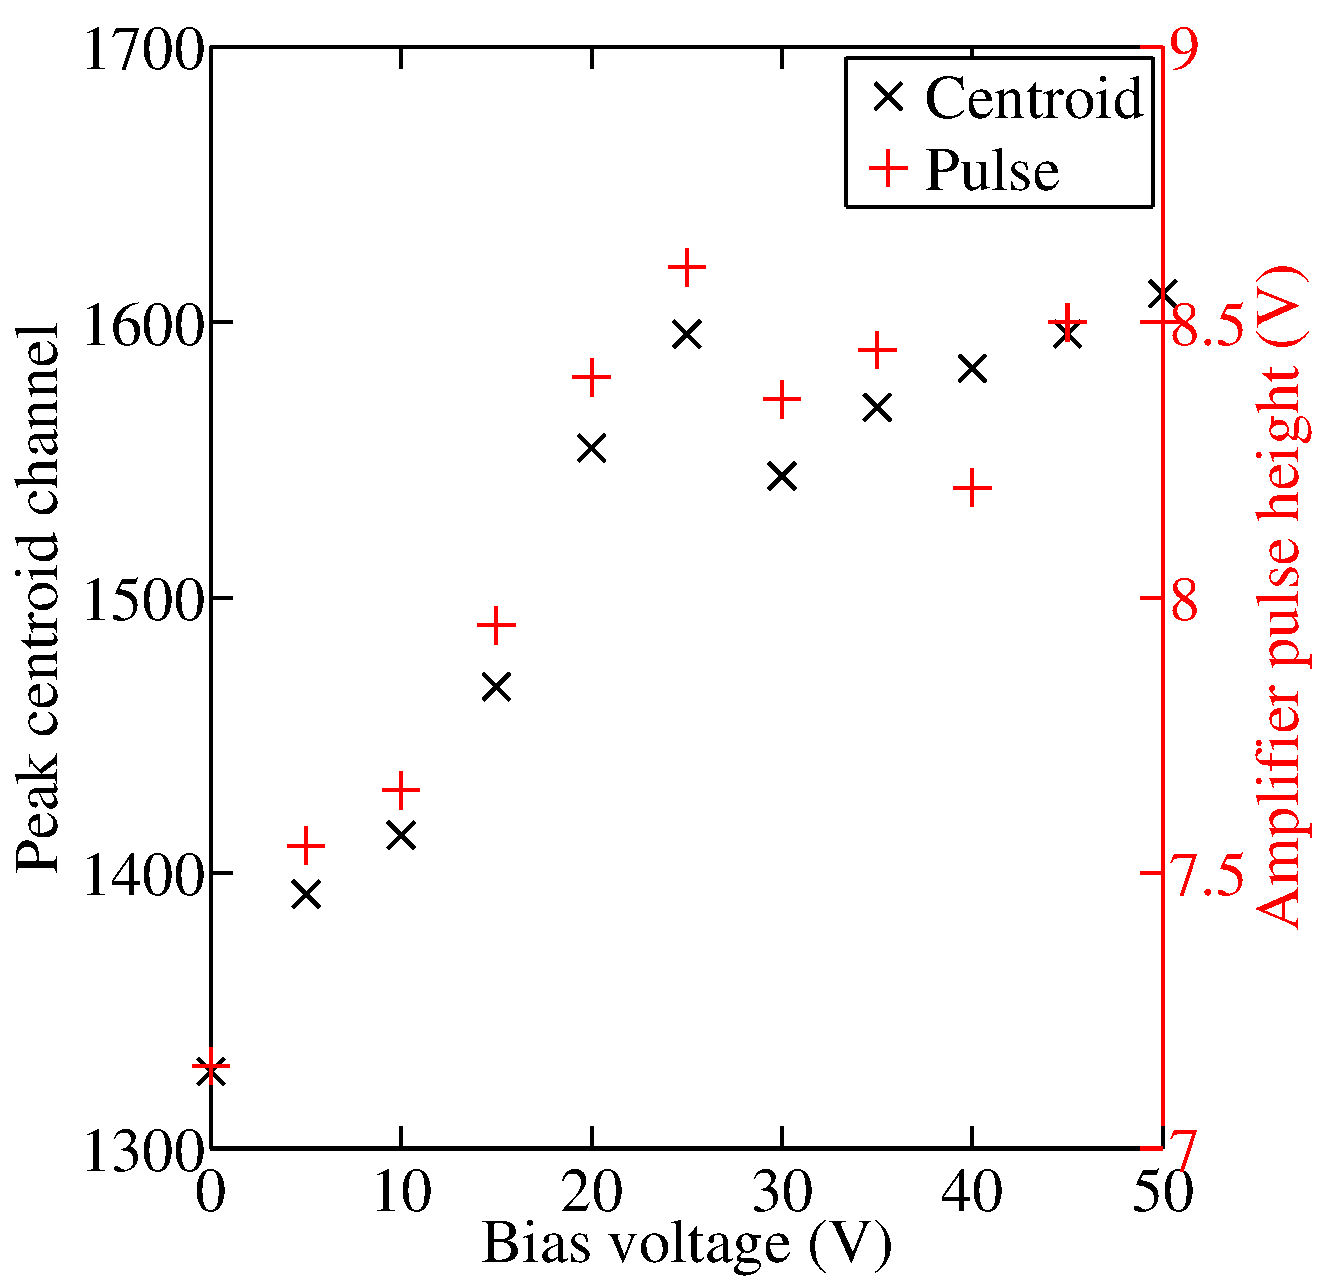
\includegraphics[width=3in]{NERS515_lab9_voltage}
  \caption{Variation of pulse height out of the amplifier with voltage.}
  \label{fig:voltage}
\end{figure}

Fig.~\ref{fig:voltage} shows the variation of pulse height as measured by the
oscilloscope and centroid channel (which should be directly proportional to the
pulse height, although less accurate) by varying the voltage across the
detector.
The discontinuity between 25 and 30 V was a result of re-pumping the vacuum
from 27 to 28.5 inHg (inches of mercury) relative to atmosphere. Aside from
that discontinuity, the curve behaves about as expected. Because the centroid
peak channel is still increasing, the detector is probably not saturated.

Incidentally, the unusual detector output when exposed to room light suggests
that the detector is a ``surface barrier'' detector, which according to Knoll
\cite[p.~377]{kno2000} are particularly sensitive to light.

%%%%%%%%%%%%%%%%%%%%%%%%%%%%%%%%%%%%%%%%%%%%%%%%%%%%%%%%%%%%%%%%%%%%%%%%%%%%%%%%
\subsection{Measured range}
The primary alpha particle released from Am-241 has an energy of 5485 keV
and a yield is 84.8\%. Another alpha with a smaller yield of 13.1\% has an
energy of 5443 keV, which is practically the same and in this problem is
neglected. The first formula gives an alpha range
$$ R = 1.24 (5.48) - 2.62 = 4.18 \units{cm}\,,$$
and the second formula gives
$$ R = (0.005 (5.48) + 2.85) (5.48)^{1.5} = 36.9 \units{mm} \,,$$
so we should expect a range of about 4 cm.
%%%%%%%%%%%%%%%%%%%%%%%%%%%%%%%%%%%%%%%%%%%%%%%%%%%%%%%%%%%%%%%%%%%%%%%%%%%%%%%%
\section{Conclusions}

We found by extrapolating the alpha's peak energy down to zero that the range
of the 5.5-MeV alpha particles is roughly 4.6 to 5.0 cm. This is only roughly
in agreement with the empirically estimated range of 3.6 to 4.2 cm.

Plotting a curve of the total alpha attenuation
should have given us a plot of the range, but the inability of the vacuum
pressure to hold at near-atmospheric levels and the geometrical aberrance
prevented a useful curve from being measured.

Finally, looking the width of the spread in alpha energies by measuring the
FWHM of the alpha peak as the pressure in the chamber changed results in a
straggling curve. As expected, the range in alpha energies increased with the
amount of material between the source and detector.

There is an abundance of sources of error in this experiment. The temperature
in the
room, which affects the air density, was not at all under control. Furthermore,
the instrumentation measuring the vacuum chamber, and the chamber itself,
were shaky at best. Another source of error was the lack of precision in the
measurement of source-detector separation; the measured distances could be off
by several millimeters at least. Finally, as is shown in
Fig.~\ref{fig:voltage}, the detector was not operated in a fully saturated,
fully depleted region. That will introduce some error into the measured MCA
spectra, since as the detector was not operated in a ``plateau'' region, the
pulse height is sensitive to changes in the high voltage bias. In fact, because
the high voltage supply is usually operated at a factor of ten to thirty higher
than in this lab, its accuracy at low voltages is questionable.
%%%%%%%%%%%%%%%%%%%%%%%%%%%%%%%%%%%%%%%%%%%%%%%%%%%%%%%%%%%%%%%%%%%%%%%%%%%%%%%%
\nocite{kno2000}
\bibliographystyle{ans}
\bibliography{bibliography}
\end{document}
